% !TEX root = ../thesis_main.tex


%%%% --- * --- %%%%	
\clearpage
\chapter{The Experimental Setup}
\label{setup_chapter}

\color{oldcolor}
\section{Overview}
The TRIUMF Neutral Atom Trap (TRINAT) offers an experimental set-up which is uniquely suited to precision tests of Standard Model beta decay physics.  Radioactive ions are delivered from the ISAC beamline and neutralized before being trapped in the first of two magneto-optical traps (MOTs).  Approximately once per second, atoms from the first MOT are transferred to the second, where their decay products can be observed with significantly less background than would have been possible in the first trap (see Figure~\ref{fig:doublemot}).  The transfer methodology is discussed in some detail in a paper by Swanson et al~\cite{swanson}. \aside{The point is that this eliminates background from the decays of other stuff.  Or the same stuff.  Stuff that's not centered at the trap.}

\begin{figure}[t!h]
	\centering
	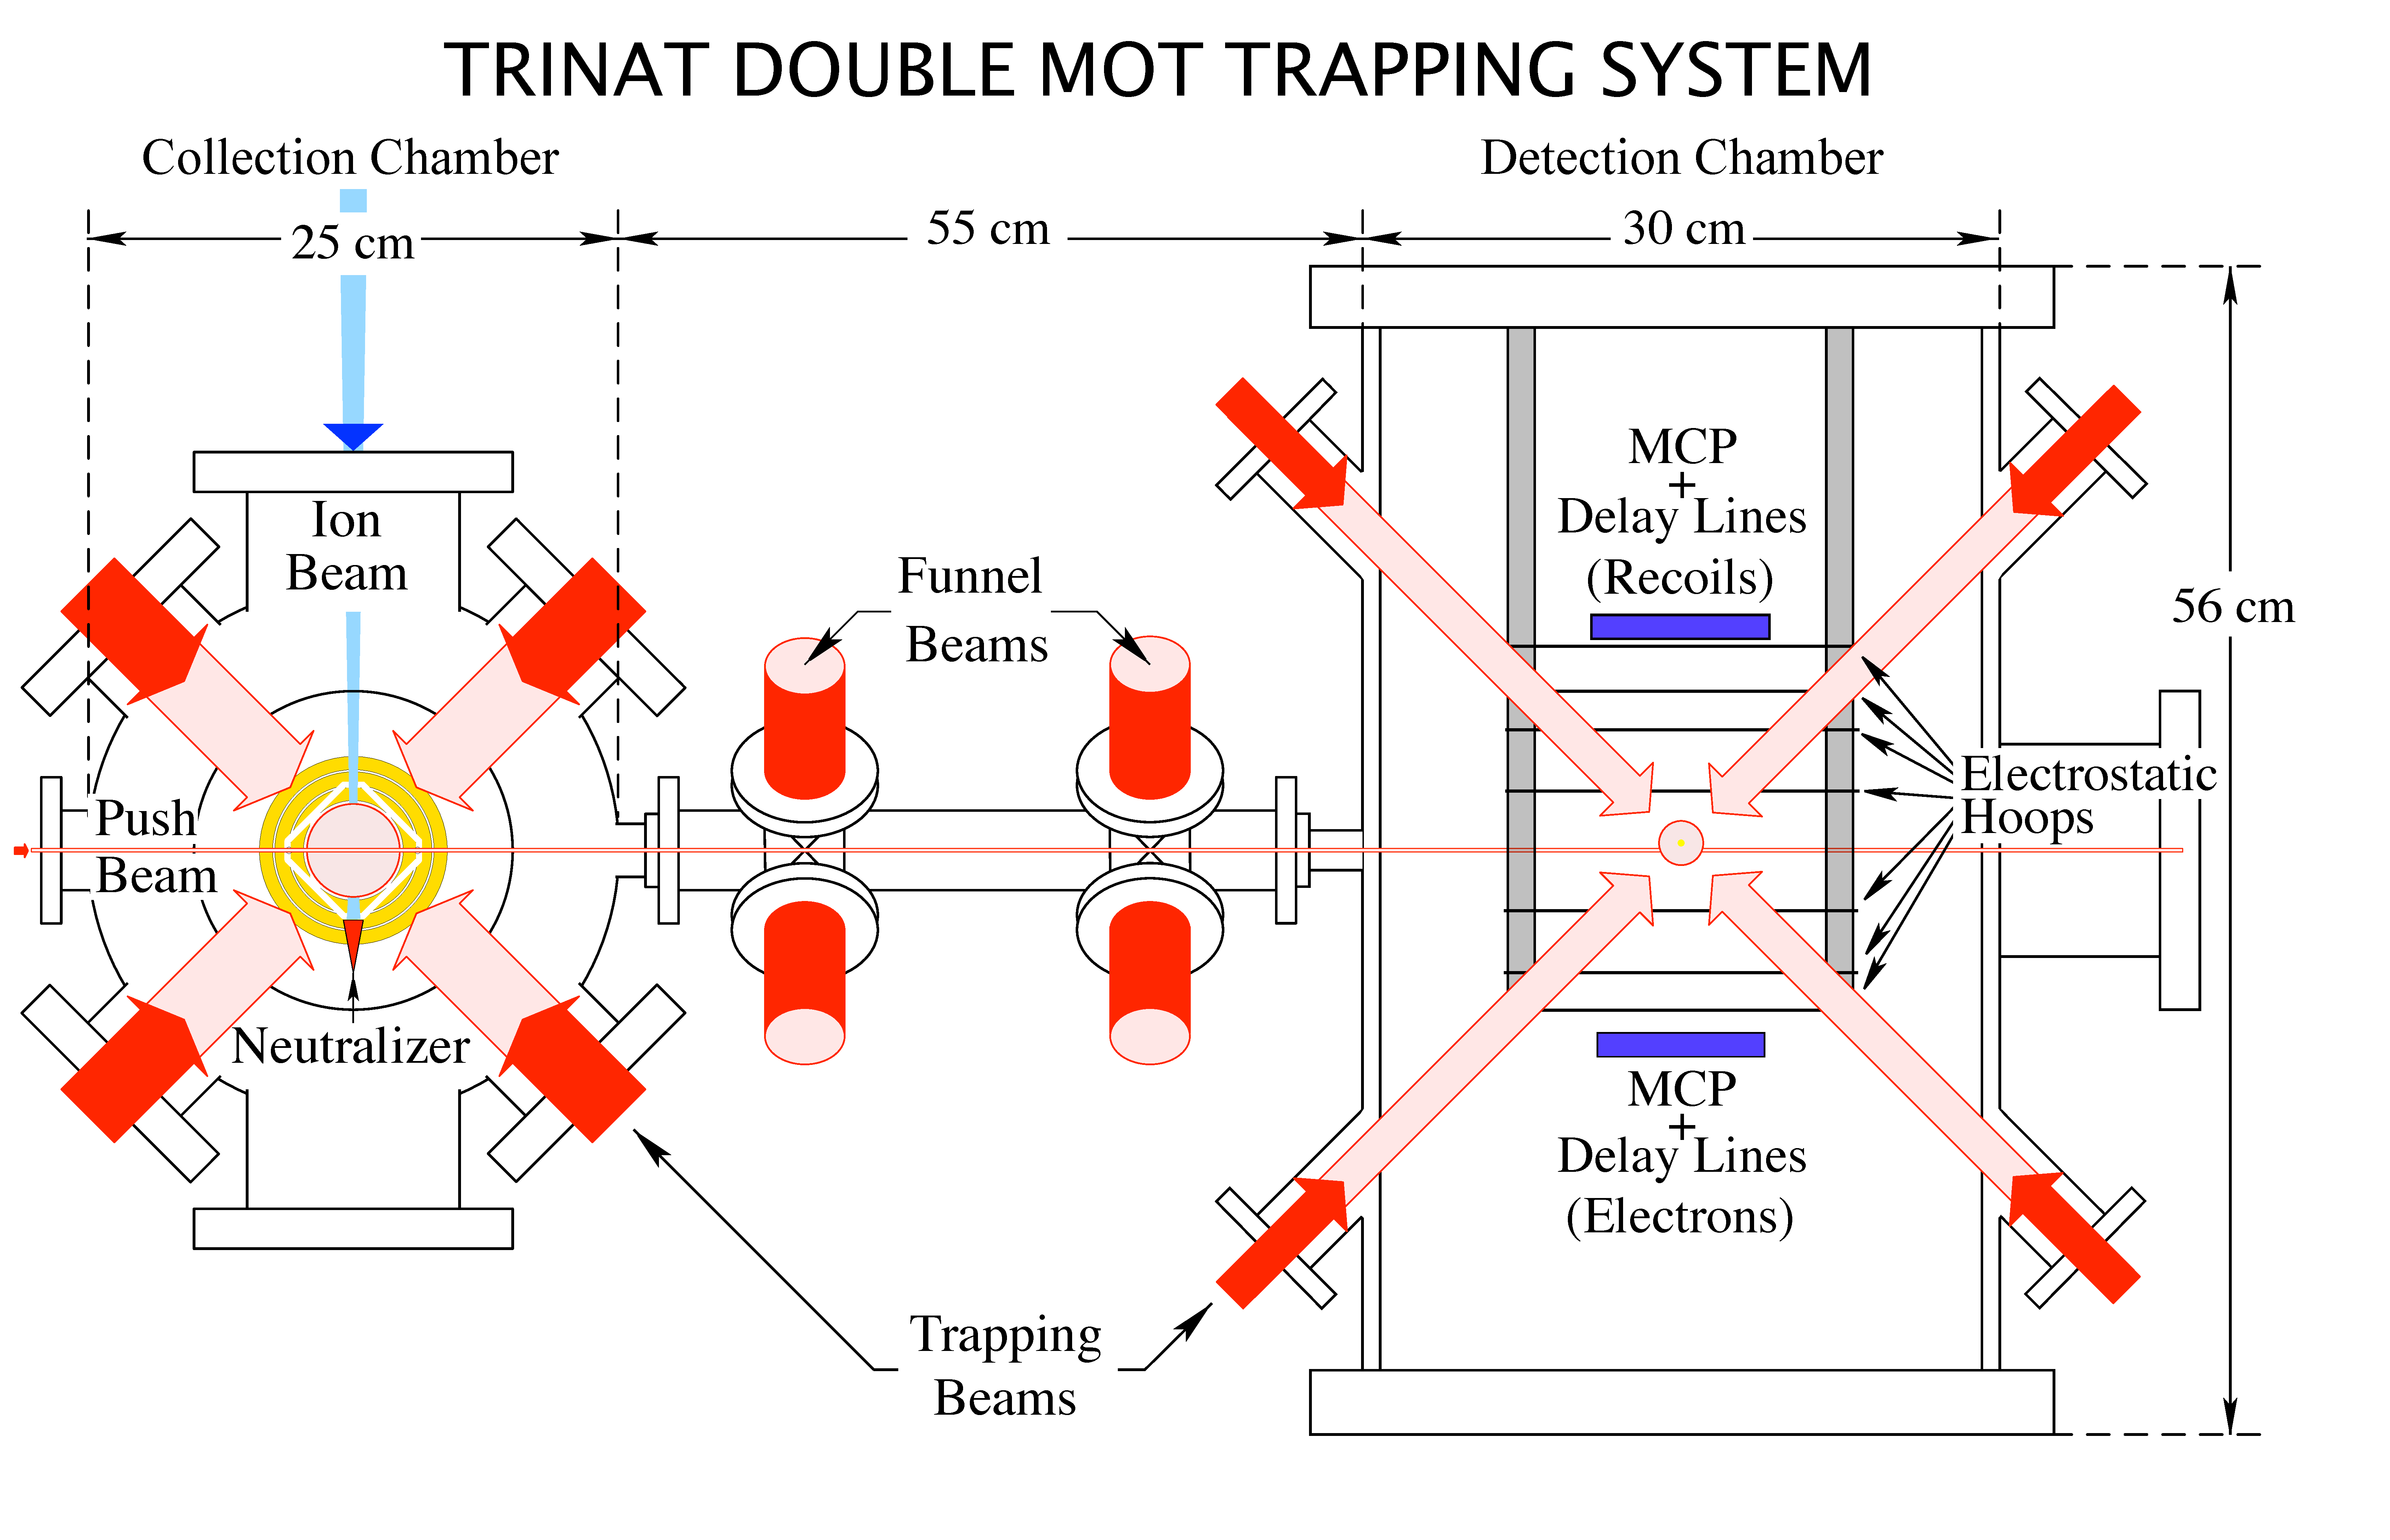
\includegraphics[width=.999\linewidth]
	{Figures/doublemot4.pdf}
	\caption{The TRINAT experimental set-up utilizes a two MOT system in order to reduce background in the detection chamber.}	
	\label{fig:doublemot}
\end{figure}

Once the newly transferred atoms -- in this case, neutral $^{37}\textrm{K}$ -- have arrived at the second trap, the MOT cycles 500 times between a state where it is `on' and actively confining atoms to a region of approximately 2\,mm$^3$, to a state where it is `off' and instead the atoms are spin-polarized by optical pumping while the atom cloud expands ballistically before being re-trapped.  In order to eliminate systematic effects, the polarization direction is flipped every 16 seconds.  This optical pumping technique and its results are the subject of a recent publication~\cite{ben_OP}.

The science chamber (shown in Figure \ref{fig:thechamber}) operates at ultra-high vacuum (UHV) and provides the apparatus necessary to intermittently confine atoms within a MOT and then spin-polarize them, and quantify their position, temperature, and initial polarization, and electrostatic hoops to allow for collection and observation of charged recoiling daughter nuclei, as well as further detectors to observe the outgoing betas and reconstruct angular correlations.  
%\comment{(should I elaborate here?) -- "no".} 

\begin{figure}[h!!!tb]
	\centering
%	\hspace*{\fill}%
	\subfloat[A decay event within the TRINAT science chamber.  After a decay, the daughter will be unaffected by forces from the MOT.  Positively charged recoils and negatively charged shake-off electrons are pulled towards detectors in opposite directions.  Although the $\beta^+$ is charged, it is also highly relativistic and escapes the electric field with minimal perturbation.
	%\comment{The pic is still kind-of fuzzy.}
	]
	{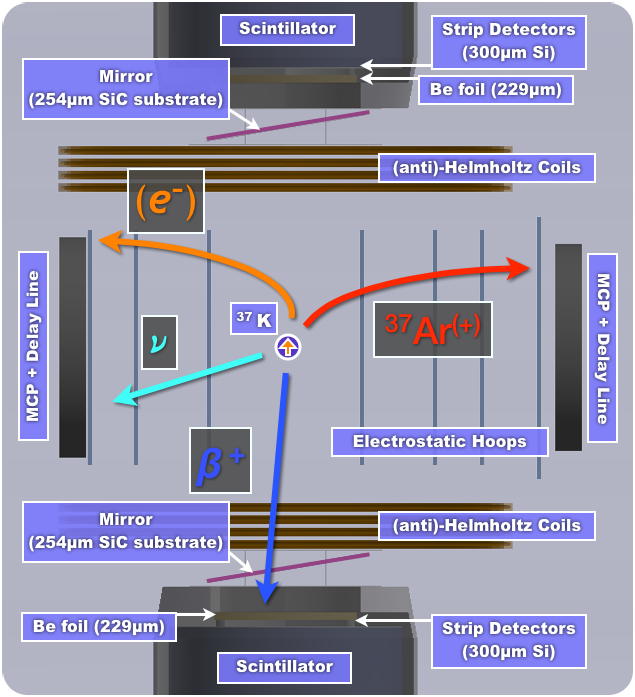
\includegraphics[width=.530\linewidth]{Figures/chamber_decayevent3.png}\label{chamber_decayevent} }
	\hspace*{\fill}
%	\hfill
	\hspace*{\fill}
	\subfloat[Inside the TRINAT science chamber.  This photo is taken from the vantage point of one of the microchannel plates, looking into the chamber towards the second microchannel plate.  The current-carrying copper Helmholtz coils and two beta telescopes are visible at the top and bottom.  The metallic piece near the center is one of the electrostatic `hoops' used to generate an electric field within the chamber.  The hoop's central circular hole allows access to the microchannel plate, and the two elongated holes on the sides allow the MOT's trapping lasers to pass unimpeded at an angle of 45 degress `out of the page'.]	
	{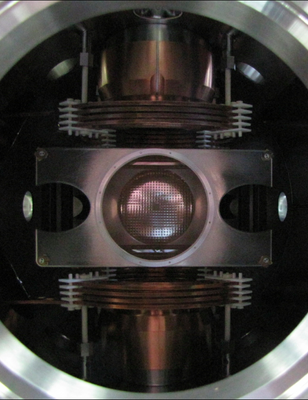
\includegraphics[width=.444\linewidth]{Figures/chamber_photo_2.png}}
%	\hspace*{\fill}%
	\caption{The TRINAT detection chamber}	
	\label{fig:thechamber}
\end{figure}
%\clearpage



\color{black}
\section{Double MOT System to Supply Atoms}
	%\\*
	Mostly, 
%	\todo{A thing that's worth noting is that (I think!) recoil-order corrections have been implicitly excluded at some point here.  ...Is this even true??}
	this requires a diagram.  We take ions supplied by the ISAC beamline, neutralize them and trap them in the first MOT, then periodically transfer them to a second MOT.  Detectors are 
%	\todo{A thing that's worth noting is that (I think!) recoil-order corrections have been implicitly excluded at some point here.  ...Is this even true??}
	positioned about the second MOT for data 
%	\lefttodo{A thing that's worth noting is that (I think!) recoil-order corrections have been implicitly excluded at some point here.  ...Is this even true??}
	collection.  This double MOT system eliminates a great deal of background.  
%	\tinytodo{A thing that's worth noting is that recoil-order corrections have been implicitly excluded at some point here. (Here's a parenthetical.) ...Is this even true??  Also, what is even happening to the spacing here??!}
	Also, here's some random equation that doesn't really go with the topic of this section:
	\bea
\frac{\partial \rho}{\partial t} &\!\!\!\!\!\! \bigg|_{relax} \!\!\! &= \:\:\: -\frac{1}{2} \left( \hat{\Gamma} \rho + \rho \,\hat{\Gamma} \right) 
\label{eq:relax} \\
\frac{\partial \rho}{\partial t} &\!\!\!\!\!\!  \bigg|_{repop} \!\!\! &= \:\:\: \hat{\Lambda},
\label{eq:repop} 
\eea

	Furthermore, here's a picture that doesn't really go with the topic of this section.
%	\lefttodo{A thing that's worth noting is that (I think!) recoil-order corrections have been implicitly excluded at some point here.  ...Is this even true??}
	collection.  This double MOT system 
	\margintodo[color=green]{A thing that's worth noting is that (I think!) recoil-order corrections have been implicitly excluded at some point here.  ...Is this even true??}
%	\todo{A thing that's worth noting is that (I think!) recoil-order corrections have been implicitly excluded at some point here.  ...Is this even true??}
	eliminates a great deal of background.  
	
%\color{oldcolor}
\section{AC-MOT and Polarization Setup}
	%\\*
	In order to facilitate a measurement of $A_{\mathrm{\beta}}$, we went to great efforts to polarize the atom cloud, and quantify that polarization.  This resulted in a duty cycle in which the atoms were intermittently trapped in the AC-MOT, then optically pumped to polarize them.  While knowledge of the polarization is less critical in a measurement of $b_{\mathrm{Fierz}}$, we still use only the polarized portion of the duty cycle in order to minimize other systematic errors, such as the scintillator energy calibration and overall trap position.
	\note[color=green]{Is that $\uparrow$ even true??  Because I'm really not sure it is.  Via Kofoedhansen, $(E_0 - E_e) = E_\nu$.  So there.}  
%	\todo[inline,color=green]{Is that $\uparrow$ even true??  Because I'm really not sure it is.  Via Kofoedhansen, $(E_0 - E_e) = E_\nu$.  So there.}
%	\todoinline[lime]{Is that $\uparrow$ even true??  Because I'm really not sure it is.  Via Kofoedhansen, $(E_0 - E_e) = E_\nu$.  So there.}  % \todo
	Anyway, here's some figures.  Or possibly one figure.  Whatever.  Also, here's a reference to a figure.  See Fig.~\ref*{fig:themot}, or also its subfigures, eg Fig.~\ref{fig:acmot} and Fig.~\ref{fig:mot}.  Maybe I have to subref them?  Like, eg, Subfig.~\subref{fig:acmot} and Subfig.~\subref*{fig:mot}.  What if we try to subref everything?  Consider, eg, Fig.~\subref{fig:themot}.
%	\todo{Does this work?  It really should.}
	\margintodo{Does this work?  It really should.}
	

	\begin{figure}[ht]
	\centering
	%	\begin{subfigure}[t]{0.237\textwidth}
		\begin{subfigure}[t]{0.242\textwidth}
			\centering
			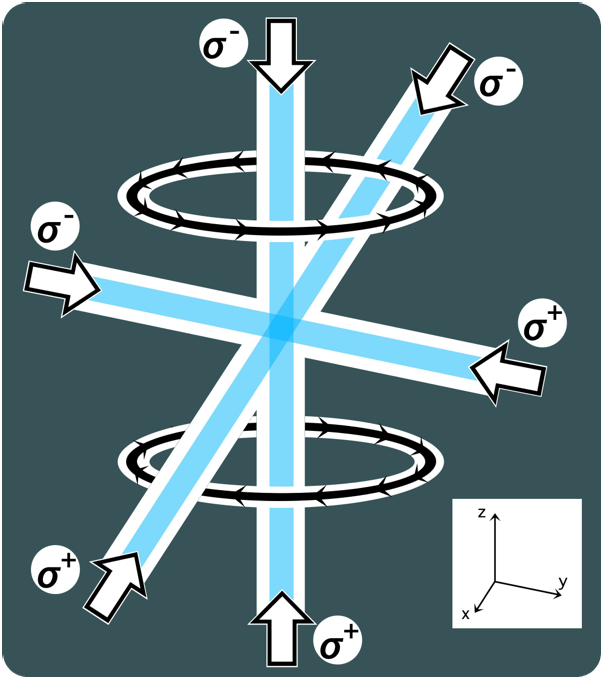
\includegraphics[width=\textwidth]{mot.png}
		%	\label{fig:mot}
			\caption{\color{oldcolor} Components of a magneto-optical trap, including current-carrying magnetic field coils and counterpropagating circularly polarized laser beams.}
			\label{fig:mot}
		\end{subfigure}
		\hfill
	%	\begin{subfigure}[t]{0.726\textwidth}
		\begin{subfigure}[t]{0.728\textwidth}
			\centering
			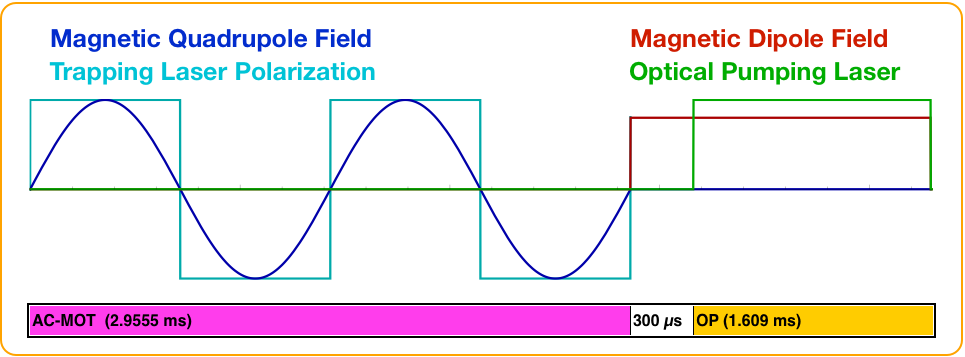
\includegraphics[width=\textwidth]{acmot.png}
			\caption{\color{oldcolor}One cycle of trapping with the AC-MOT, followed by optical pumping to spin-polarize the atoms.  After atoms are transferred into the science chamber, this cycle is repeated 500 times before the next transfer.  The magnetic dipole field is created by running parallel (rather than anti-parallel as is needed for the MOT) currents through the two coils.}
			\label{fig:acmot}
		\end{subfigure}
		\caption{\color{oldcolor}An alternating-current magneto-optical trap with a duty cycle optimized for producing polarized atoms}	
		\label{fig:themot}
	\color{black}
	\end{figure}
	
	
	
%\color{black}
%	\subsection{\textbf{Nuclear Setup}}
\section{Measurement Geometry and Detectors}
	%\\*
	Needs several diagrams.  Back-to-back beta detectors along the polarization axis.  Back-to-back MCPs in an electric field to tag events from the trap, and to measure the trap position and polarization.  Hoops to produce the electric field.  Many laser ports to make the MOT functional, and for optical pumping.  Fancy mirror geometry to combine optical pumping and trapping light along the vertical axis.  Water-cooled (anti-)Helmholz coils within the chamber for the AC-MOT, fast switching to produce an optical pumping field.  
%	\subsection{\textbf{All the Detectors}}

